% I2SB talk: guided diffusion as posterior ascent, warm starts, and the bridge.
% Built from immap_guided_ascent.tex. Compile with pdflatex (twice).
\documentclass[aspectratio=169, 11pt]{beamer}

\usetheme[progressbar=frametitle, numbering=fraction]{metropolis}
\usefonttheme[onlymath]{serif}

\usepackage{amsmath, amssymb, mathtools, bm}
\usepackage{booktabs, array}
\usepackage{tikz}
\usepackage{pgfplots}
\pgfplotsset{compat=1.17}
\usepackage{algpseudocode}
\usetikzlibrary{arrows.meta, calc, decorations.pathreplacing}

\newcommand{\x}{\bm{x}}
\newcommand{\y}{\bm{y}}
\newcommand{\z}{\bm{z}}
\newcommand{\uu}{\bm{u}}
\newcommand{\eps}{\bm{\varepsilon}}
\newcommand{\hx}{\hat{\bm{x}}}
\newcommand{\tx}{\tilde{\bm{x}}}
\newcommand{\E}{\mathbb{E}}
\newcommand{\N}{\mathcal{N}}
\newcommand{\Op}{\bm{E}}
\newcommand{\ssb}{\sigma_{\mathrm{sb}}}
\newcommand{\D}{D}

\definecolor{ca}{RGB}{31, 119, 180}   % blue
\definecolor{cb}{RGB}{23, 140, 120}   % teal
\definecolor{cc}{RGB}{214, 110, 20}   % orange
\definecolor{cmean}{RGB}{180, 40, 60}    % red: the posterior mean
\setbeamercolor{alerted text}{fg=cc}

\title{I\textsuperscript{2}SB as guided posterior ascent}
\subtitle{Guided diffusion, warm starts, and the bridge}
\author{ImMAP project}
\date{November 2026}

\begin{document}

\maketitle

%=============================================================================================
\begin{frame}{Three ideas}
\begin{enumerate}
  \setlength{\itemsep}{10pt}
  \item \textbf{Guided diffusion is gradient ascent on the posterior.}\\
        Guess the image, step part of the way toward the guess, add back a little less noise,
        repeat.
  \item \textbf{A warm start skips the useless first steps.}\\
        Start from a likely image plus noise instead of from pure noise.
  \item \textbf{A bridge is the same ascent in better coordinates.}\\
        When the guide is paired with the target, connect them by a bridge of noisy images.
        I\textsuperscript{2}SB is then the ascent, line by line, with a better-conditioned
        network input.
\end{enumerate}
\end{frame}

%=============================================================================================
\section{Guided diffusion as posterior ascent}
%=============================================================================================

\begin{frame}{The problem}
\begin{itemize}
  \setlength{\itemsep}{6pt}
  \item Recover an image $\x$ from \alert{side information} $\y$ about it: a paired scan of
        another contrast (a guide), a measurement, or both.
  \item Our case, knee MRI: $\x$ is the PDFS scan; $\y$ is the PD guide and the undersampled
        PDFS $k$-space.
  \item Probabilistically, we want the most likely image given what we know:
        \[
          \hx = \arg\max_{\x}\ \log p(\x\mid\y).
        \]
  \item An end-to-end network (TGVN, LGGS) regresses $\E[\x\mid\y]$ in one shot: the
        \emph{average} of every image consistent with $\y$. Sharp where $\y$ pins $\x$ down,
        blurry where it does not.
\end{itemize}
\end{frame}

%---------------------------------------------------------------------------------------------
\begin{frame}{Smooth the objective, then anneal}
\begin{columns}[T]
\begin{column}{0.47\textwidth}
\begin{itemize}
  \setlength{\itemsep}{6pt}
  \item Noisy targets $\z = \x + \sigma\eps$ have density
        \[
          p_\sigma(\z\mid\y) = \textstyle\int \N(\z;\x,\sigma^2\bm I)\,p(\x\mid\y)\,d\x .
        \]
  \item \textbf{Large $\sigma$}: one broad hill, easy to climb.
  \item \textbf{$\sigma\to0$}: the posterior itself, with many sharp peaks.
  \item Climb at a large $\sigma$ and lower it as you go (ImMAP, Kadkhodaie \& Simoncelli
        2021).
\end{itemize}
\end{column}
\begin{column}{0.51\textwidth}
\centering
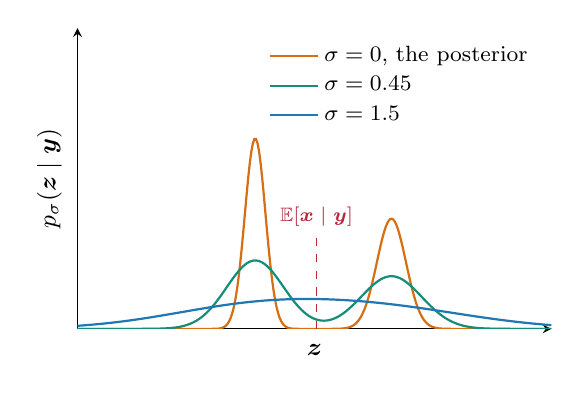
\begin{tikzpicture}[
  declare function={g(\t,\m,\v) = exp(-(\t-\m)^2/(2*\v))/sqrt(2*pi*\v);
                    p(\t,\s) = 0.55*g(\t,-1,0.03+\s*\s) + 0.45*g(\t,1.3,0.06+\s*\s);}]
\begin{axis}[width=7.6cm, height=5.4cm, domain=-4:4, samples=301, axis lines=left,
             xtick=\empty, ytick=\empty, ymin=0, ymax=2.0, xlabel={$\z$},
             ylabel={$p_\sigma(\z\mid\y)$}, every axis label/.style={font=\small},
             legend style={draw=none, font=\footnotesize, at={(0.98,0.98)}, anchor=north east},
             legend cell align=left]
  \addplot[thick, cc]  {p(x,0)};    \addlegendentry{$\sigma = 0$, the posterior}
  \addplot[thick, cb]  {p(x,0.45)}; \addlegendentry{$\sigma = 0.45$}
  \addplot[thick, ca]  {p(x,1.5)};  \addlegendentry{$\sigma = 1.5$}
  \draw[dashed, cmean] (axis cs:0.04,0) -- (axis cs:0.04,0.62)
        node[above, font=\scriptsize, cmean] {$\E[\x\mid\y]$};
\end{axis}
\end{tikzpicture}
\end{column}
\end{columns}
\end{frame}

%---------------------------------------------------------------------------------------------
\begin{frame}{A denoiser is the gradient}
\textbf{Tweedie's formula.} With $\D(\z,\sigma,\y) \coloneqq \E[\x\mid\z,\y]$ at noise level
$\sigma$,
\[
  \sigma^2\,\nabla_{\z}\log p_\sigma(\z\mid\y) = \D(\z,\sigma,\y) - \z .
\]
So a network trained to denoise, given $\y$, hands us the gradient of the smoothed objective.

\medskip
\textbf{One gradient step} with step size $h\sigma^2$:
\[
  \boxed{\ \z^+ = (1-h)\,\z + h\,\D(\z,\sigma,\y)\ }
  \qquad\text{move the fraction $h$ of the way toward the guess.}
\]
Every $h\in(0,2)$ increases $\log p_\sigma$.

\medskip
\textbf{Then re-noise.} The step leaves noise $(1-h)\sigma$. Inject fresh noise $\gamma\eps$ so
the iterate is again a noisy target, at the next, smaller level $\sigma' = r\sigma$:
\[
  \gamma^2 = \sigma'^2 - (1-h)^2\sigma^2 .
\]
\end{frame}

%---------------------------------------------------------------------------------------------
\begin{frame}{One run, step by step}
\begin{columns}[T]
\begin{column}{0.56\textwidth}
\centering
\begin{tikzpicture}[scale=1.08, >=Stealth, font=\footnotesize]
  \useasboundingbox (-0.2,-0.4) rectangle (7.4,4.4);
  \clip (-0.2,-0.4) rectangle (7.4,4.4);
  % the posterior: two modes
  \fill[cc!25] (5.05,1.0) ellipse (0.45 and 0.22);
  \fill[cc!25] (6.3,2.7) ellipse (0.35 and 0.3);
  \node[cc!80!black, anchor=west] at (5.55,0.85) {likely};
  \node[cc!80!black] at (6.3,3.2) {likely};
  % step 1: start
  \only<1->{
    \draw[ca, dashed] (0.8,3.6) circle (2.9);
    \fill[ca] (0.8,3.6) circle (2pt) node[above right] {$\z_N$};
  }
  % step 2: first guess = posterior mean
  \only<2->{
    \draw[->, ca, thick] (0.8,3.6) -- (5.6,1.87);
    \fill[cmean] (5.67,1.85) circle (2.2pt) node[right, cmean] {$\E[\x\mid\y]$};
  }
  % step 3: partial step and re-noise
  \only<3->{
    \fill[gray] (3.62,2.52) circle (1.3pt);
    \draw[->, gray] (3.62,2.52) -- (3.52,1.98);
    \draw[cb, dashed] (3.5,1.9) circle (1.4);
    \fill[cb] (3.5,1.9) circle (2pt) node[above left] {$\z_{N-1}$};
  }
  % step 4
  \only<4->{
    \draw[->, cb, thick] (3.5,1.9) -- (4.85,1.37);
    \fill[cmean!70] (4.9,1.35) circle (1.8pt);
    \fill[gray] (4.34,1.57) circle (1.3pt);
    \draw[->, gray] (4.34,1.57) -- (4.44,1.28);
    \draw[cc, dashed] (4.45,1.25) circle (0.6);
    \fill[cc] (4.45,1.25) circle (2pt);
  }
  % step 5
  \only<5->{
    \fill[cmean!50] (4.97,1.04) circle (1.6pt);
    \draw[->, cc, thick] (4.45,1.25) -- (4.92,1.06);
    \fill[black] (5.02,1.0) circle (2pt) node[below right=-1pt] {$\hx$};
  }
\end{tikzpicture}
\end{column}
\begin{column}{0.42\textwidth}
\small
\begin{itemize}
  \setlength{\itemsep}{3pt}
  \item<1-| alert@1> \textbf{Start in pure noise:} an unlikely image that says nothing beyond
        $\y$. Circle: noise level $\sigma$.
  \item<2-| alert@2> \textbf{Guess} $\approx\E[\x\mid\y]$, the end-to-end answer: an average,
        \emph{between} the likely images.
  \item<3-| alert@3> \textbf{Step part of the way}, add back less noise: a little more likely.
  \item<4-| alert@4> \textbf{Guess again} at lower $\sigma$. The noise has committed us to one
        option, so the guess is sharper.
  \item<5-| alert@5> \textbf{As $\sigma\to0$} the guess lands on a likely image.
\end{itemize}
\end{column}
\end{columns}
\end{frame}

%---------------------------------------------------------------------------------------------
\begin{frame}{Annealed posterior ascent}
\begin{columns}[T]
\begin{column}{0.5\textwidth}
\begin{algorithmic}[1]
\Require denoiser $\D$; start $\z$ at level $\sigma$ ($\infty$ allowed)
\While{$\sigma > \sigma_{\min}$}
  \State $\hx \gets \D(\z,\sigma,\y)$ \Comment{guess}
  \State choose $h$, $r$ with $|1-h|\le r$
  \State $\z \gets (1-h)\,\z + h\,\hx + \gamma\,\eps$ \Comment{step}
  \State $\sigma \gets r\sigma$
\EndWhile
\State \Return $\hx$
\end{algorithmic}
\end{column}
\begin{column}{0.48\textwidth}
\small
Three step sizes worth naming:
\begin{itemize}
  \item $h = 1-r^2$: the ancestral (DDPM / VE) sampler. Returns a posterior sample.
  \item $h = 1-r$: no noise injected; the probability-flow ODE. Climbs to the MAP.
  \item $h = 1$: jump to the guess and re-noise (SDEdit restarts).
\end{itemize}
\end{column}
\end{columns}

\bigskip
\begin{alertblock}{The first step from $\sigma=\infty$}
$r=0$ forces $h=1$: the step returns $\D(\cdot,\infty,\y) = \E[\x\mid\y]$, whatever $\z$ was,
and re-noises it. An end-to-end network is exactly this first step, without the rest.
\end{alertblock}
\end{frame}

%=============================================================================================
\section{Warm starts}
%=============================================================================================

\begin{frame}{Cold starts are wasteful}
\begin{itemize}
  \item At the top of the ladder ($\sigma\gg$ image intensities) the iterate is almost all
        noise, and every guess is $\approx\E[\x\mid\y]$.
  \item Those steps rebuild a blur we could have computed once.
\end{itemize}
\bigskip
\centering
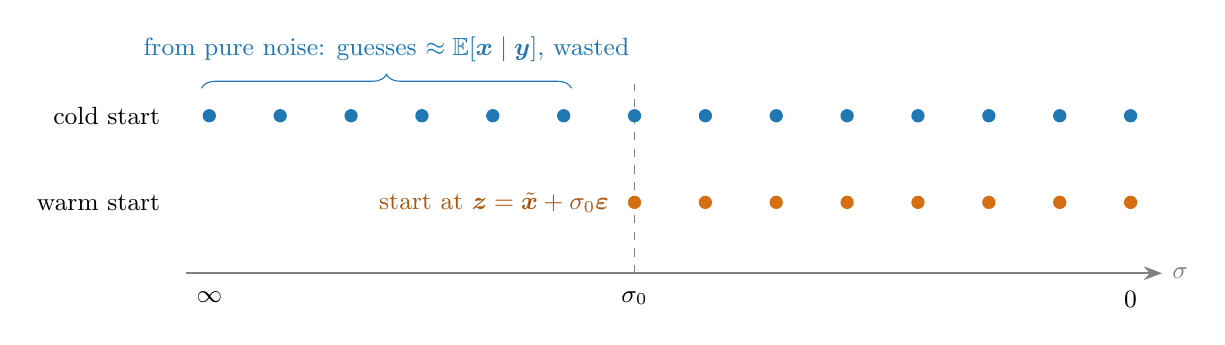
\begin{tikzpicture}[>=Stealth, font=\small]
  \draw[->, thick, gray] (0,-0.9) -- (12.4,-0.9) node[right] {$\sigma$};
  \node[below=3pt] at (0.3,-0.9) {$\infty$};
  \node[below=3pt] at (12,-0.9) {$0$};
  \draw[dashed, gray] (5.7,-0.9) -- (5.7,1.5);
  \node[below=3pt] at (5.7,-0.9) {$\sigma_0$};
  % cold
  \node[anchor=east] at (-0.2,1.1) {cold start};
  \foreach \p in {0.3,1.2,2.1,3.0,3.9,4.8,5.7,6.6,7.5,8.4,9.3,10.2,11.1,12.0}
    \fill[ca] (\p,1.1) circle (2.4pt);
  \draw[decorate, decoration={brace, amplitude=5pt}, ca] (0.2,1.45) -- (4.9,1.45)
        node[midway, above=6pt, ca] {from pure noise: guesses $\approx\E[\x\mid\y]$, wasted};
  % warm
  \node[anchor=east] at (-0.2,0) {warm start};
  \foreach \p in {5.7,6.6,7.5,8.4,9.3,10.2,11.1,12.0}
    \fill[cc] (\p,0) circle (2.4pt);
  \node[anchor=east, cc!80!black] at (5.5,0) {start at $\z = \tx + \sigma_0\eps$};
\end{tikzpicture}
\end{frame}

%---------------------------------------------------------------------------------------------
\begin{frame}{Start from a likelier image}
\begin{itemize}
  \setlength{\itemsep}{6pt}
  \item Sample a likelier image and add noise: $\z = \tx + \sigma_0\eps$, with $\sigma_0<\infty$.
        Then run the same ascent from $\sigma_0$: fewer steps, at little cost
        (SDEdit; come-closer-diffuse-faster).
  \item Candidates for $\tx$:
        \begin{itemize}
          \item the adjoint (zero-filled) image $\Op^H\y$;
          \item an end-to-end reconstruction, $\approx\E[\x\mid\y]$.
        \end{itemize}
  \item \textbf{Choosing $\sigma_0$.} The noise must cover the start's error:
        $\sigma_0 \gtrsim$ RMS error of $\tx$. Too little, and the run cannot leave $\tx$'s
        neighbourhood.
  \item The ascent from $\sigma=\infty$ is itself warm-started: its first step re-noises
        $\E[\x\mid\y]$. ImMAP2 starts at $\mathrm{mean}(\Op^H\y)+\z$, $\sigma=1$.
\end{itemize}
\end{frame}

%---------------------------------------------------------------------------------------------
\begin{frame}{The start level matters}
\small
CIFAR-10, $4\times$ super-resolution, one trained guided denoiser, 8 samples $\times$ 512 images.
\emph{Detail}: energy in the band the low-res input cannot see, relative to the target's
(perfect sample $=1$; the regression $\E[\x\mid\y]$ has $0.29$).

\medskip
\centering
\begin{tabular}{@{}lcccc@{}}
\toprule
start & \multicolumn{2}{c}{10 network calls} & \multicolumn{2}{c}{50 network calls} \\
\cmidrule(lr){2-3}\cmidrule(l){4-5}
 & sample spread & detail & sample spread & detail \\
\midrule
$\sigma=\infty$, then re-noise (I\textsuperscript{2}SB)      & 0.084 & 0.49 & 0.122 & 0.71 \\
$\E[\x\mid\y] + \sigma_0\eps$, $\sigma_0\approx2.0$       & 0.105 & 0.60 & 0.130 & 0.76 \\
$\E[\x\mid\y] + \sigma_0\eps$, $\sigma_0=0.5$             & 0.078 & 0.46 & 0.088 & 0.51 \\
\bottomrule
\end{tabular}

\medskip
\raggedright
$\sigma_0 = 0.5$ is about $3\times$ the regression's RMS error, and still too low: samples
plateau near the regression even at 50 calls. Warm, but not too warm.
\end{frame}

%=============================================================================================
\section{Specialising to a bridge}
%=============================================================================================

\begin{frame}{A paired guide: build a bridge}
\begin{columns}[T]
\begin{column}{0.55\textwidth}
\small
\begin{itemize}
  \setlength{\itemsep}{4pt}
  \item Suppose the guide $\y$ is \alert{uniquely paired} with the target $\x$.
  \item Connect them by a \textbf{Brownian bridge}, a distribution of noisy paths from $\x$
        to $\y$:
        \[
          \begin{gathered}
            \z_t = (1-t)\,\x + t\,\y + \ssb(t)\,\eps,\\
            \ssb(t)^2 = V t(1-t).
          \end{gathered}
        \]
  \item $t=0$: the target. $t=1$: exactly the guide. Noise at most $\tau = \sqrt V/2$.
  \item A Schr\"odinger bridge between the two image distributions. With paired data each
        pair's endpoints are pinned, and it is this Gaussian bridge (Liu et al.\ 2023).
\end{itemize}
\end{column}
\begin{column}{0.43\textwidth}
\centering
\vspace{0.8cm}
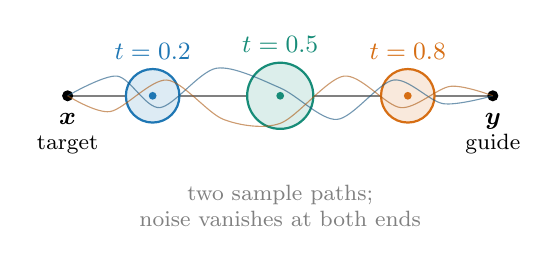
\begin{tikzpicture}[>=Stealth, font=\small]
  \draw[gray, thick] (0,0) -- (5.4,0);
  \fill (0,0) circle (2pt) node[below=3pt, align=center] {$\x$\\[-2pt]{\footnotesize target}};
  \fill (5.4,0) circle (2pt) node[below=3pt, align=center] {$\y$\\[-2pt]{\footnotesize guide}};
  \foreach \t/\r/\c in {0.2/0.34/ca, 0.5/0.42/cb, 0.8/0.34/cc} {
    \fill[\c!15] (5.4*\t, 0) circle (\r);
    \draw[\c, thick] (5.4*\t, 0) circle (\r);
    \fill[\c] (5.4*\t, 0) circle (1.4pt);
    \node[\c, above] at (5.4*\t, \r) {$t = \t$};
  }
  % two sample paths
  \begin{scope}[opacity=0.6, xscale=0.9]
    \draw[ca!70!black] plot[smooth] coordinates {(0,0) (0.7,0.25) (1.3,-0.15) (2.1,0.35)
          (3.0,0.1) (3.8,-0.3) (4.6,0.2) (5.3,-0.1) (6,0)};
    \draw[cc!80!black] plot[smooth] coordinates {(0,0) (0.6,-0.2) (1.4,0.2) (2.2,-0.3)
          (3.0,-0.35) (3.9,0.25) (4.7,-0.15) (5.4,0.12) (6,0)};
  \end{scope}
  \node[font=\footnotesize, gray, align=center] at (2.7,-1.4) {two sample paths;\\
        noise vanishes at both ends};
\end{tikzpicture}

\vspace{0.8cm}
\small
\textbf{Training:} predict the target,
\[
  \min_{\D}\ \E\,\|\D(\z_t,t,\y)-\x\|^2,\quad t\sim\mathcal U[0,1].
\]
\end{column}
\end{columns}
\end{frame}

%---------------------------------------------------------------------------------------------
\begin{frame}{Same skeleton: guess, step, re-noise onto the bridge}
\begin{columns}[T]
\begin{column}{0.48\textwidth}
\textbf{Guided diffusion}
\begin{algorithmic}[1]
\State $\z \gets$ pure noise
\For{each level $\sigma\to\sigma'$}
  \State $\hx \gets \D(\z,\sigma,\y)$
  \State $\z \gets (1-h)\z + h\hx + \gamma\eps$
\EndFor
\end{algorithmic}
\end{column}
\begin{column}{0.5\textwidth}
\textbf{I\textsuperscript{2}SB}
\begin{algorithmic}[1]
\State $\z \gets \y$ \Comment{the guide}
\For{each time $t\to s$, $\ s<t$}
  \State $\hx \gets \D(\z,t,\y)$
  \State $\z \gets \tfrac st\,\z + \big(1-\tfrac st\big)\hx + \sqrt{V\tfrac{s(t-s)}{t}}\,\eps$
\EndFor
\end{algorithmic}
\end{column}
\end{columns}

\bigskip
\begin{itemize}
  \item \textbf{Re-noising onto the bridge.} Line 4 draws the bridge from the guess $\hx$ (at
        time 0) to the current point $\z$ (at time $t$), at the earlier time $s$.
  \item The first step: $\z = \y$ and the guess is $\E[\x\mid\y]$, a regression from the guide.
        Then step down the bridge toward the target.
\end{itemize}
\end{frame}

%---------------------------------------------------------------------------------------------
{\setbeamercolor{background canvas}{bg=black!85}
\begin{frame}[standout]
The bridge is a change of coordinates.\\[8pt]
{\normalsize I\textsuperscript{2}SB is the posterior ascent, run through a better network input.}
\end{frame}}

%---------------------------------------------------------------------------------------------
\begin{frame}{Debias the bridge}
\begin{columns}[T]
\begin{column}{0.44\textwidth}
\small
Remove the guide's share and rescale:
\[
  \uu = \frac{\z_t - t\,\y}{1-t} = \x + \sigma(t)\,\eps,
\]
\[
  \sigma(t)^2 = \frac{Vt}{1-t}.
\]
\begin{itemize}
  \setlength{\itemsep}{3pt}
  \item $\uu$ is a noisy target: what the ascent iterates on.
  \item For fixed $\y$ the map is a bijection, so
        $\E[\x\mid\z_t,\y] = \E[\x\mid\uu,\y]$. The bridge network \emph{is} the guided
        denoiser.
  \item Bridge time is the noise level: $t=0\mapsto\sigma=0$, $t=1\mapsto\sigma=\infty$.
\end{itemize}
\end{column}
\begin{column}{0.54\textwidth}
\centering
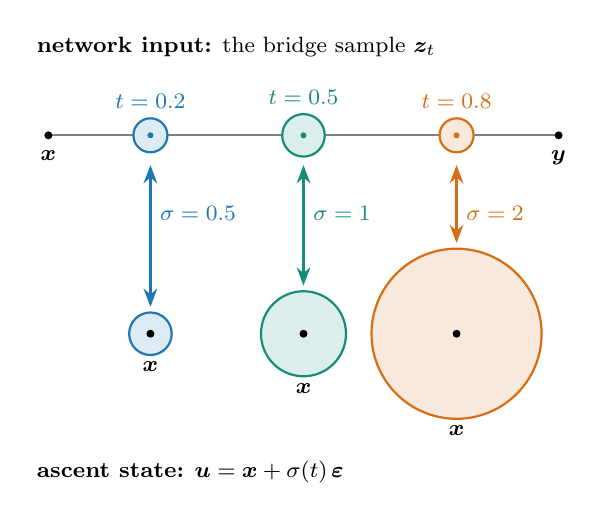
\begin{tikzpicture}[>=Stealth, font=\footnotesize, scale=0.9]
  \node[anchor=west] at (-0.3, 1.25) {\textbf{network input:} the bridge sample $\z_t$};
  \draw[gray, thick] (0,0) -- (7.2,0);
  \fill (0,0) circle (1.6pt) node[below=2pt] {$\x$};
  \fill (7.2,0) circle (1.6pt) node[below=2pt] {$\y$};
  \foreach \t/\r/\c in {0.2/0.24/ca, 0.5/0.30/cb, 0.8/0.24/cc} {
    \fill[\c!15] (7.2*\t, 0) circle (\r);
    \draw[\c, thick] (7.2*\t, 0) circle (\r);
    \fill[\c] (7.2*\t, 0) circle (1.2pt);
    \node[\c, above] at (7.2*\t, \r) {$t = \t$};
  }
  \node[anchor=west] at (-0.3, -4.75) {\textbf{ascent state:} $\uu = \x + \sigma(t)\,\eps$};
  \foreach \t/\r/\c/\s in {0.2/0.30/ca/0.5, 0.5/0.60/cb/1, 0.8/1.20/cc/2} {
    \fill[\c!15] (7.2*\t, -2.8) circle (\r);
    \draw[\c, thick] (7.2*\t, -2.8) circle (\r);
    \fill (7.2*\t, -2.8) circle (1.6pt);
    \node[below=-1pt] at (7.2*\t, -2.8 - \r) {$\x$};
    \draw[<->, \c, thick] (7.2*\t, -0.42) -- (7.2*\t, -2.8 + \r + 0.08);
  }
  \node[ca, right] at (1.44, -1.1) {$\sigma = 0.5$};
  \node[cb, right] at (3.60, -1.1) {$\sigma = 1$};
  \node[cc, right] at (5.76, -1.1) {$\sigma = 2$};
\end{tikzpicture}

{\scriptsize Same state, two coordinates (radii to scale, $V=1$).}
\end{column}
\end{columns}
\end{frame}

%---------------------------------------------------------------------------------------------
\begin{frame}{Line by line}
\footnotesize
Grid $1 = t_N>\dots>t_0 = 0$; $t=t_k$, $s=t_{k-1}$; $r^2 = \sigma(s)^2/\sigma(t)^2 =
\frac{s(1-t)}{t(1-s)}$; the same noise $\eps_k$ in both.

\medskip
\begin{columns}[T]
\begin{column}{0.47\textwidth}
\textbf{Ascent in $\uu$}, with $h = 1-r^2$
\begin{algorithmic}[1]
\State $\uu \gets$ anything \Comment{$\sigma_N=\infty$}
\For{$k = N,\dots,1$}
  \State $\hx \gets \D\big(\y + (1-t)(\uu-\y),\,t,\,\y\big)$
  \State $\uu \gets r^2\uu + (1-r^2)\,\hx + \sigma(s)\sqrt{1-r^2}\,\eps_k$
\EndFor
\State \Return $\uu$
\end{algorithmic}
\end{column}
\begin{column}{0.5\textwidth}
\textbf{I\textsuperscript{2}SB in $\z$}
\begin{algorithmic}[1]
\State $\z \gets \y$
\For{$k = N,\dots,1$}
  \State $\hx \gets \D(\z,\,t,\,\y)$
  \State $\z \gets \tfrac st\,\z + \big(1-\tfrac st\big)\hx + \sqrt{V\tfrac{s(t-s)}{t}}\,\eps_k$
\EndFor
\State \Return $\z$
\end{algorithmic}
\end{column}
\end{columns}

\medskip
\begin{itemize}
  \item \textbf{Line 1.} At $t=1$ the input $\y + 0\cdot(\uu-\y)$ is $\y$, whatever $\uu$ is.
  \item \textbf{Line 3.} The left input is $\z_t$, so the guesses are equal.
  \item \textbf{Line 4.} Multiply by $1-s$ and add $s\y$: the coefficients become
        $\tfrac st$, $1-\tfrac st$, and the variance
        $(1-s)^2\sigma(s)^2(1-r^2) = V\tfrac{s(t-s)}{t}$.
\end{itemize}
\end{frame}

%---------------------------------------------------------------------------------------------
\begin{frame}{Checked on a trained network}
\centering
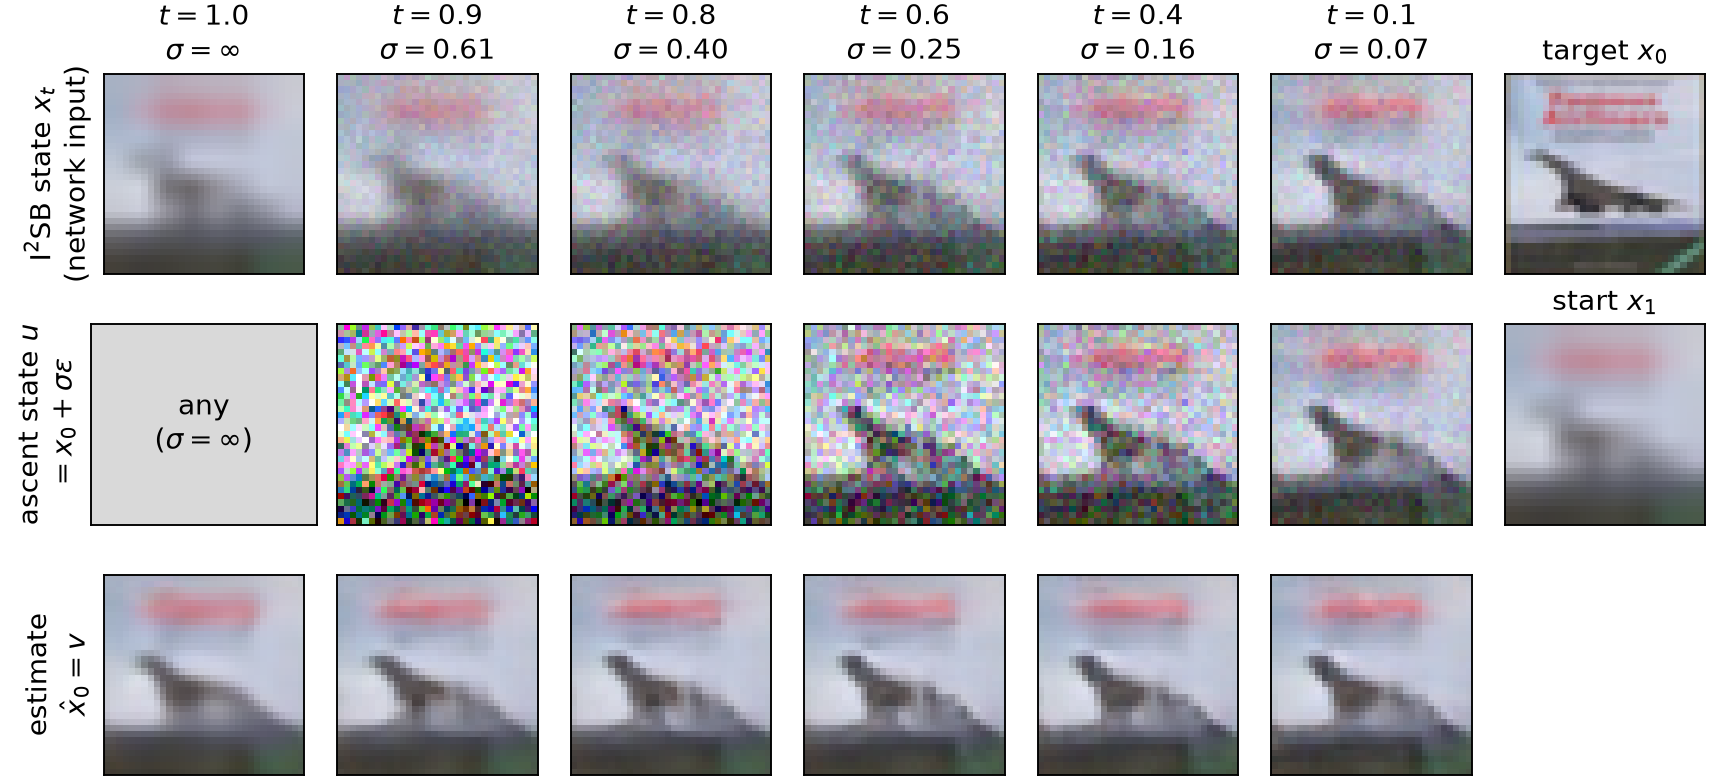
\includegraphics[width=0.86\textwidth]{equivalence_toy/trajectory.png}

\small
\raggedright
One I\textsuperscript{2}SB run (CIFAR $4\times$ SR), both coordinates, same noise. Over 256 images
the two algorithms agree to $7.6\cdot10^{-7}$ relative (5 steps) and $7.8\cdot10^{-7}$
(50 steps): float32 rounding. They are one computation.
\end{frame}

%---------------------------------------------------------------------------------------------
\begin{frame}{So why a bridge?}
\small
The optimal outputs are equal, so in theory nothing is gained. But a finite network must fit the
denoiser at every level, and the bridge removes the levels where that is hardest.
\begin{itemize}
  \setlength{\itemsep}{2pt}
  \item \textbf{Bounded noise.} The network sees noise $\ssb(t)\le\tau$, while $\sigma$ runs
        from $0$ to $\infty$.
  \item \textbf{Exact start.} At $\sigma=\infty$ the input is exactly $\y$, an image it is
        trained on. Standard diffusion stops at a finite $\sigma_{\max}$ and starts from
        mismatched noise.
  \item \textbf{A Wiener-filter preconditioner.} $\z_t = \y + (1-t)(\uu-\y)$ is
        $\E[\x\mid\uu]$ under the prior $\x\sim\N(\y,V\bm I)$. The network only learns the
        correction, and the better $\y$ predicts $\x$, the smaller it is.
\end{itemize}

\medskip
\footnotesize
\centering
\begin{tabular}{@{}lll@{}}
\toprule
 & conditional diffusion (EDM) & bridge (I\textsuperscript{2}SB) \\
\midrule
ideal denoiser & $\E[\x\mid\uu,\sigma,\y]$ & the same \\
network input & $c_{\mathrm{in}}(\sigma)\,\uu$ & $\y + (1-t)(\uu-\y)$ \\
top level, start & finite $\sigma_{\max}$, pure noise & $\sigma=\infty$, the guide $\y$ \\
\bottomrule
\end{tabular}
\end{frame}

%---------------------------------------------------------------------------------------------
\begin{frame}{Where it pays: very few steps}
\small
Same CIFAR task. Two networks, same architecture, data and budget: the bridge network, and a
standard conditional diffusion network (EDM). Consistency is the RMSE against the measurement
($\times10^{-3}$, lower is better).

\medskip
\centering
\begin{tabular}{@{}lcccc@{}}
\toprule
 & \multicolumn{4}{c}{consistency, by network calls} \\
\cmidrule(l){2-5}
 & 2 & 3 & 5 & 50 \\
\midrule
bridge net, I\textsuperscript{2}SB ladder from $\y$  & \textbf{10.3} & 10.5 & 10.8 & 11.9 \\
bridge net, $\sigma$-ladder from noise          & \textbf{10.3} & 10.2 & 10.5 & 13.1 \\
EDM net, $\sigma$-ladder from noise             & 42.5 & 17.3 & 10.9 & 9.4 \\
EDM net, I\textsuperscript{2}SB ladder               & 18.2 & 14.2 & 11.1 & 9.9 \\
\bottomrule
\end{tabular}

\medskip
\raggedright
\begin{itemize}
  \item With 2 calls the EDM network fails: its first guess, at $\sigma=80$, is poor.
  \item The bridge network is accurate up to $\sigma=\infty$, so it works from $\y$ or from
        noise.
  \item From 5 calls on the curves merge. I\textsuperscript{2}SB's edge is low step counts.
\end{itemize}
\end{frame}

%---------------------------------------------------------------------------------------------
\begin{frame}{From the guide or from noise: the same posterior}
\centering
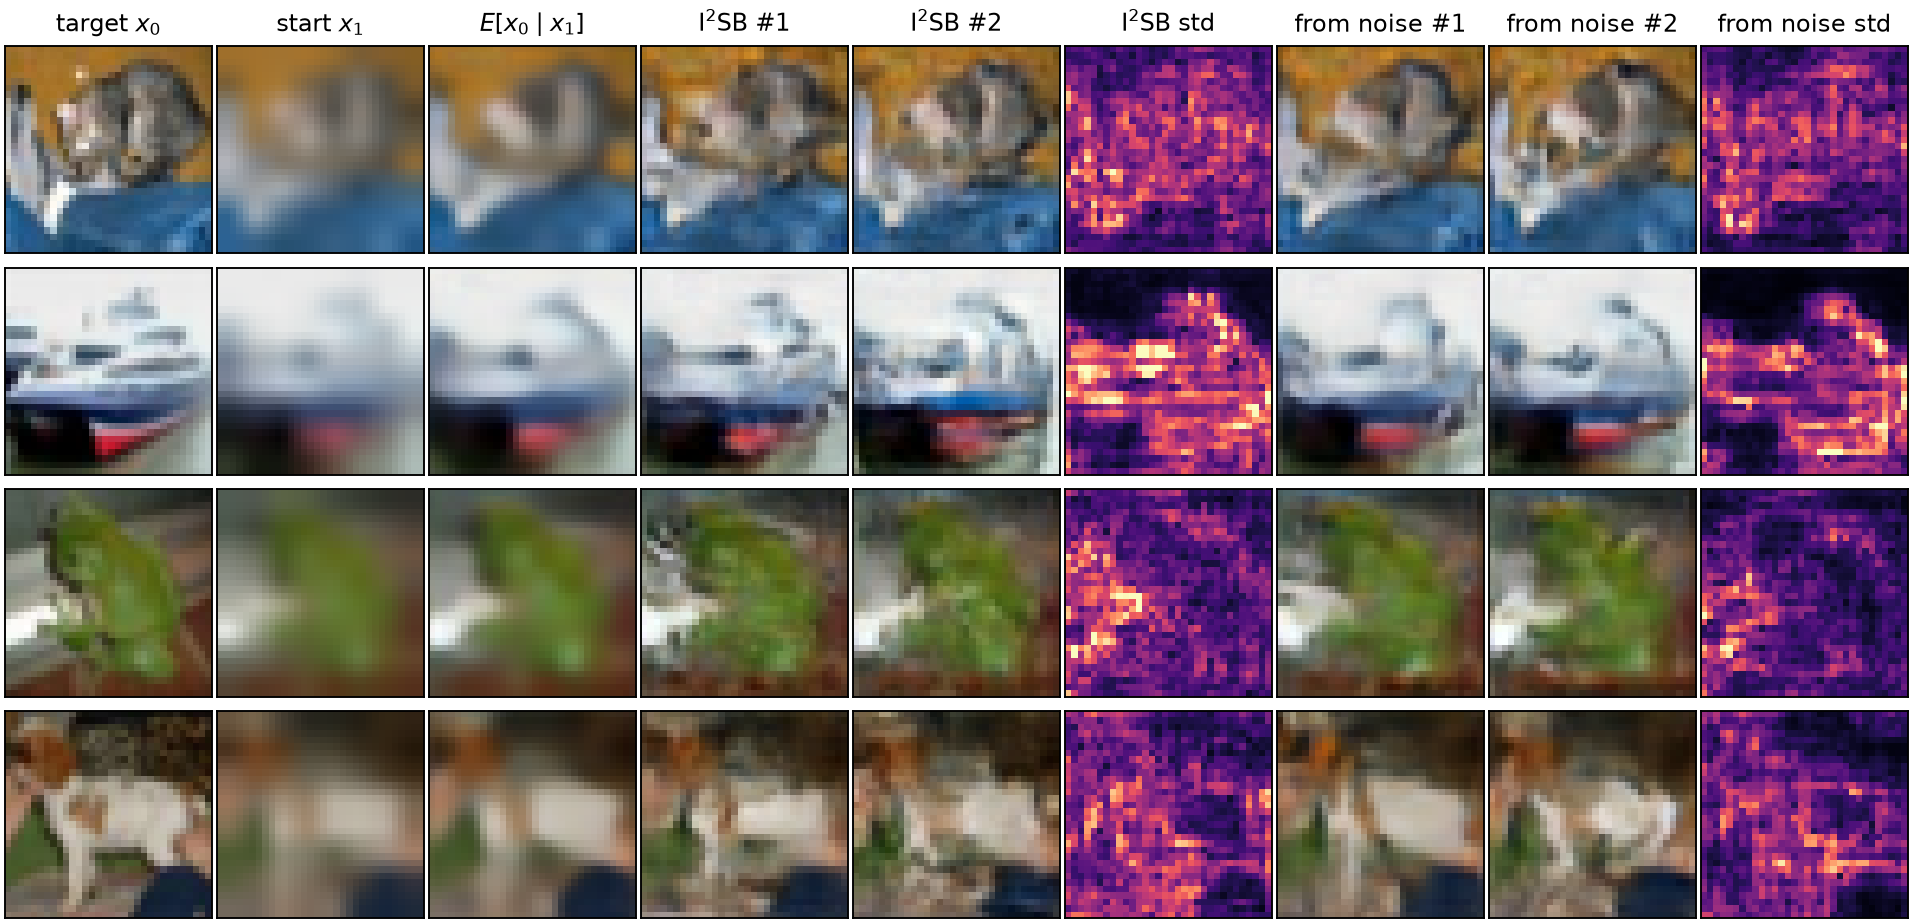
\includegraphics[width=0.76\textwidth]{equivalence_toy/samples_top4.png}

\small
\raggedright
Same bridge network, 50 steps, 8 samples per image (512 images). From $\y$ (I\textsuperscript{2}SB)
or from pure noise at $\sigma=80$, the posterior means differ by $0.92\times$ the Monte-Carlo
noise and the spreads agree to 0.2\%; retraining the network moves results about as much.
Starting at $\y$ is the $\sigma=\infty$ end of the same ascent.
\end{frame}

%---------------------------------------------------------------------------------------------
\begin{frame}{Takeaways}
\begin{enumerate}
  \setlength{\itemsep}{8pt}
  \item Guided diffusion is annealed gradient ascent on $\log p(\x\mid\y)$: guess with a
        denoiser, step part of the way, add back less noise. Its first step from
        $\sigma=\infty$ is the end-to-end network.
  \item A warm start, $\tx + \sigma_0\eps$, skips the steps that only rebuild $\E[\x\mid\y]$.
        $\sigma_0$ must still cover the start's error.
  \item With a paired guide, I\textsuperscript{2}SB is that same ascent in bridge coordinates,
        line for line. The bridge changes the network's input and training, not the target.
        It pays when steps are few.
\end{enumerate}
\end{frame}

%=============================================================================================
\appendix
\section*{Backup}
%=============================================================================================

\begin{frame}{Backup: every method is one ascent}
\footnotesize
\centering
\begin{tabular}{@{}>{\raggedright\arraybackslash}p{3.6cm}>{\raggedright\arraybackslash}p{2.0cm}%
                >{\raggedright\arraybackslash}p{4.4cm}>{\raggedright\arraybackslash}p{3.6cm}@{}}
\toprule
method & conditions on & estimator of the guess & ladder, step \\
\midrule
SDEdit & nothing & unconditional denoiser; guide only in the start & free \\
ImMAP2 & measurement & data step on an unconditional denoiser & self-paced; $\beta=0.05$ \\
I\textsuperscript{2}SB & guide & bridge regressor & fixed; $h = 1-r^2$ \\
I\textsuperscript{2}SB-Recon / -Inversion & guide, meas. & data step on the bridge regressor &
  as I\textsuperscript{2}SB, 80 steps \\
TGVN, LGGS end-to-end & guide, meas. & learned $\E[\x\mid\y]$ & one step from $\sigma=\infty$ \\
\bottomrule
\end{tabular}

\bigskip
\raggedright
\small
\textbf{ImMAP2 vs.\ I\textsuperscript{2}SB-Recon.} Not comparable as such: one is given the guide,
the other is not. With a zero-filled start $\Op^H\y$ (sufficient for the measurement under
Gaussian noise) the objectives coincide, and the two differ only in estimator and schedule.
\end{frame}

\end{document}
